\section{Theory}
\subsection{Constant Deviation Spectrometer}
An instrument used to study the spectra with an unaided eye is called a spectroscope or spectrometer. For this experiment, a constant deviation prism of the angle of minimum deviation $90 \degree$ is used such that the emission spectrum can be observed from a telescope placed perpendicular to the source and collimator (incident beam). For this purpose, the prism comprises three parts: two $30 \degree$ prisms, PQR and QTS, and the reflecting prism PRS as shown in the figure below. When the angle of incidence is equal to the angle of emergence and the
the angle of deviation is $90 \degree$, a ray would be passing through a position of minimum deviation. 

\begin{figure}[H]
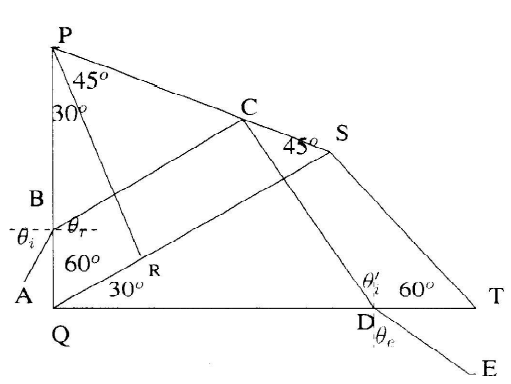
\includegraphics[height=3.5cm, width=6cm]{MP2.png}
\caption{\textbf{Constant deviation Prism}}
\label{fig1}
\end{figure}

\subsection{Emission spectra of metals}
To observe the absorption spectra of the metals, the apparatus needs to be calibrated first. For this purpose, a mercury lamp of known wavelength and spectrum is used as a source. The experimental setup consists of the source, a collimator and the constant deviation prism. A telescope is placed perpendicular to the collimator to observe the spectra as shown in \hyperref[fig:2]{Figure 2}. The cylinder has markings on it. We will fix the cylinder at the 546nm mark (the green light, because it is almost at the middle of the spectrum: this way we would be able to reduce the error). We have to place the prism on the table in such a way that the green band almost coincides with the crosshair. Next, we have to take the values of different wavelengths and calibrate the device markings with the actual measurements. For the spectra of metals, the metal source will be heated and placed in front of the collimator. The heating will excite the electrons and further de-excitation will produce the emission spectra.


\begin{figure}[H]
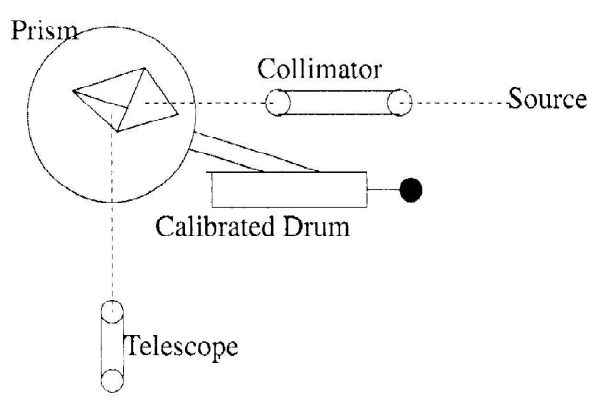
\includegraphics[height=4cm, width=7cm]{MP3.png}
\caption{\textbf{Experimental Setup}}
\label{fig:2}
\end{figure}

\subsection{Absorption Spectrum of Iodine Vapour}
The iodine absorption spectrum can be explained by vibronic transitions between the energy levels of different quantum states defined by their vibrational quantum numbers. For this experiment, Iodine vapours are excited by a source of white light and missing (absorbed) wavelengths of light are observed in the spectrum which appear as dark bands. The absorption involves the following transition: $(X, \nu'') \rightarrow (B, \nu')$\\
where X represents the ground state and B is the first excited electronic energy state. $\nu'' (=0, 1, 2\; etc)$ and $\nu' (=0,1,2,\; etc)$ represent the vibrational quantum numbers in the ground and excited electronic states, respectively.\\
As shown in the figure, for transitions between the ground state and the first excited state at room temperature, the first transition corresponds to $\nu'' =0$ to $\nu' = 0$ which is labelled as the $0\leftarrow0$ absorption line.\\

\begin{figure}[H]
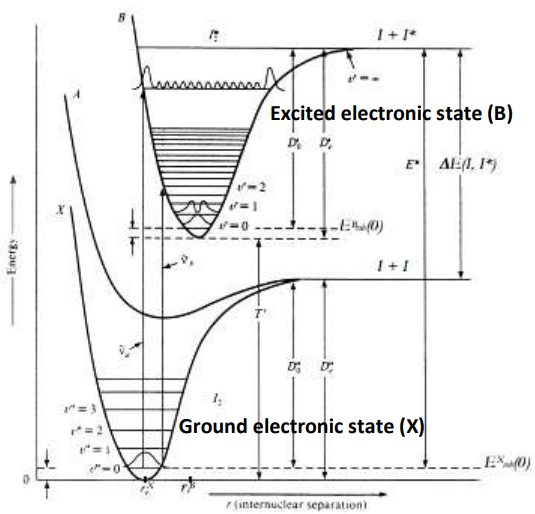
\includegraphics[height=8cm, width=8cm]{MP4.png}
\caption{\textbf{Schematic energy level diagram of iodine}}
\label{fig3}
\end{figure}

According to the Franck-Condon principle, only those wavefunctions of the two stat don't significantly overlap with the ground state wavefunction, therefore usually the transition from $20\; to\;50\leftarrow0$ takes place. For the maximum energy level, $\nu_{max}$ the energies form a continuum rather than being quantized and hence bond dissociation occurs given by:
$$(D_0)=\;E(\nu'=\nu_{max})-E(\nu'=0)$$

Since the vibronic energy levels are coarsely placed, one can apply the simple harmonic oscillator equations involving Morse potential to solve for energy levels, giving the force constant to be: 
$$f=4\pi^2 \mu\;(c\Delta\bar{\nu_{e^{avg}}})^2$$
